\documentclass[%
	%draft,
	%submission,
	%compressed,
	final, %technote,
	%internal,
	%submitted,
	%inpress,
	%reprint,
	% %titlepage,
	notitlepage,
	%anonymous,
	narroweqnarray,
	inline,
	twoside,
        %invited,
	]{ieee}

\usepackage[top=3cm, bottom=2cm, left=1.5cm, right=1.5cm,a4paper,includeheadfoot]{geometry}



\usepackage[utf8]{inputenc}			% idioma
\usepackage[spanish]{babel}
\usepackage{float}
%\usepackage{color}
%\usepackage{colortbl}
%\usepackage{amsmath}
%\usepackage{amsfonts}
%\usepackage{verbatim}

\usepackage{hyperref}				% urls

% -------- PARA FIGURAS
\usepackage{graphicx}
%\usepackage{capt-of}
% -------- FIN FIGURAS

% -------- PARA MONXTRAR EL CODIGO DE MANERA AMENA
\usepackage{courier}
\usepackage{listings}
\lstset{ %
	language=C++,                % choose the language of the code
	basicstyle=\footnotesize\ttfamily,       % the size of the fonts that are used for the code
	numbersep=5pt,                  % how far the line-numbers are from the code
%	backgroundcolor=\color{white},  % choose the background color. You must add \usepackage{color}
	showspaces=false,               % show spaces adding particular underscores
	showstringspaces=false,         % underline spaces within strings
	showtabs=false,                 % show tabs within strings adding particular underscores
	frame=single,           % adds a frame around the code
	tabsize=6,          % sets default tabsize to 2 spaces
	captionpos=b,           % sets the caption-position to bottom
	breaklines=true,        % sets automatic line breaking
	breakatwhitespace=false,    % sets if automatic breaks should only happen at whitespace
}
% -------- FIN CODIGO

\hypersetup{			%sacar los colores horrendos de las ref
	colorlinks=false,
	pdfborder={0 0 0},
}


\begin{document}


\title[Rutas en redes]{%
  Rutas en redes: Utilizando traceroute y m\'etodos estadísticos para detectar enlaces submarinos
}

\author[CIRUELOS, MADDONNI, PATAN\'E, THIBEAULT]{
Gonzalo Ciruelos \authorinfo{G. Ciruelos e-mail: gonzalo.ciruelos@gmail.com}%
\and{}Axel Maddonni \authorinfo{A. Maddonni, e-mail: axel.maddonni@gmail.com}%
\and{}Federico Patan\'e \authorinfo{F. Patan\'e, e-mail: fedepatane20@gmail.com}%
\and{}Gabriel Thibeault \authorinfo{G. Thibeault, e-mail: gabriel.eric.thibeault@gmail.com}
}

\journal{Grupo 13: Teor\'ia de las Comunicaciones, Departamento de Computaci\'on, UBA}

\firstpage{1}

\maketitle               


\begin{abstract} 
  Bla bla
\end{abstract}

\begin{keywords}
  Bla, bla, bla
\end{keywords}


\section{Introducci\'on te\'orica}

\PARstart En este trabajo nos proponemos usar un traceroute junto con herramientas estadísticas para intentar detectar enlaces submarinos en las rutas IP. 

Nuestra implementación de traceroute se basará en paquetes ICMP de tipo \texttt{echo request}. Enviaremos, al destino especificado, paquetes ICMP echo request con distintos TTL, esperando que el paquete se quede sin tiempo en un nodo intermedio, y este nodo intermedio nos mande otro paquete ICMP (esta vez de tipo \texttt{time exceeded}) y de esta manera sabremos la dirección IP del nodo intermedio.


Más adelante introduciremos más en detalle cómo fue hecha la implementación de traceroute. Sin embargo, lo que más nos interesa del traceroute es el RTT entre cada nodo: como podemos tomar el tiempo que tarda un paquete en ir y volver de cada nodo intermedio de la ruta, podemos estimar el tiempo que tarda el salto entre cada nodo de la ruta. De esta manera, como nuestro objetivo es detectar enlaces submarinos, podemos pensar que una buena forma de detectarlos sería detectar cuando el salto tarda mucho.

Esto es efectivamente lo que haremos, tendremos una variable aleatoria que será el RTT relativo, es decir, entre saltos, y tomaremos todos los RTT relativos de nuestro traceroute como muestras de esa variable aleatoria. Luego, usando algún modelo de detección de outliers, intentaremos detectar mediciones que corresponden con enlaces submarinos.

Como método de detección de outliers utilizaremos el método descripto en \cite{outliers}. Este método se basa en normalizar la variable aleatoria, para obtener una nueva variable aleatoria que llamaremos ZRTT. Es decir, supondremos que los RTT relativos son una $N(\mu, \sigma)$ para algún $\mu$, $\sigma$ y normalizaremos para obtener una $N(0,1)$.

\[
  ZRTT = \frac{RTT_i - \overline{RTT}}{s_{RTT}}
\]

Notar que sin embargo este método es imperfecto, porque la variable aleatoria podría no ser (y de hecho no es) una normal.

Ahora bien, tenemos que elegir algún valor límite tal que si $ZRTT$ es mayor que ese valor, diremos que es un outlier, y en consecuencia ese enlace es un enlace submarino. Aquí, es donde el paper \cite{outliers} propone utilizar la variable $\tau$ de Thompson. La $\tau$ de Thompson se calcula como sigue

\[
  \tau = \frac{
                 t_{\frac{\alpha}{2}} (n-1)
              }{
                 \sqrt{n} \sqrt{n-2 + t_{\frac{\alpha}{2}}^2}
              }
\]

Donde $n$ es la cantidad de mediciones. 

Todo esto resume la parte teórica del problema. De aquí en adelante nos adentraremos en la implementación de la herramienta, y en la experimentación.






\section{Desarrollo}

\PARstart Como explicamos anteriormente, \ldots


\subsection{Primera consigna}

\subsection{Segunda consigna}

\par Cabe destacar que en el cálculo de los ZRTTs, sólo tomamos valores no-negativos\footnote{Consideramos como 0 a los valores negativos.} de los RTTs entre saltos. 
Sin embargo, en los gráficos de RTTs que presentamos, los valores pueden ser menores a 0.
De forma contraria las figuras proveen información confusa y difícil de interpretar.

\subsection{Conceptos generales}


\subsection{Ōsaka daigaku}


\begin{figure}[H]
    \centering
    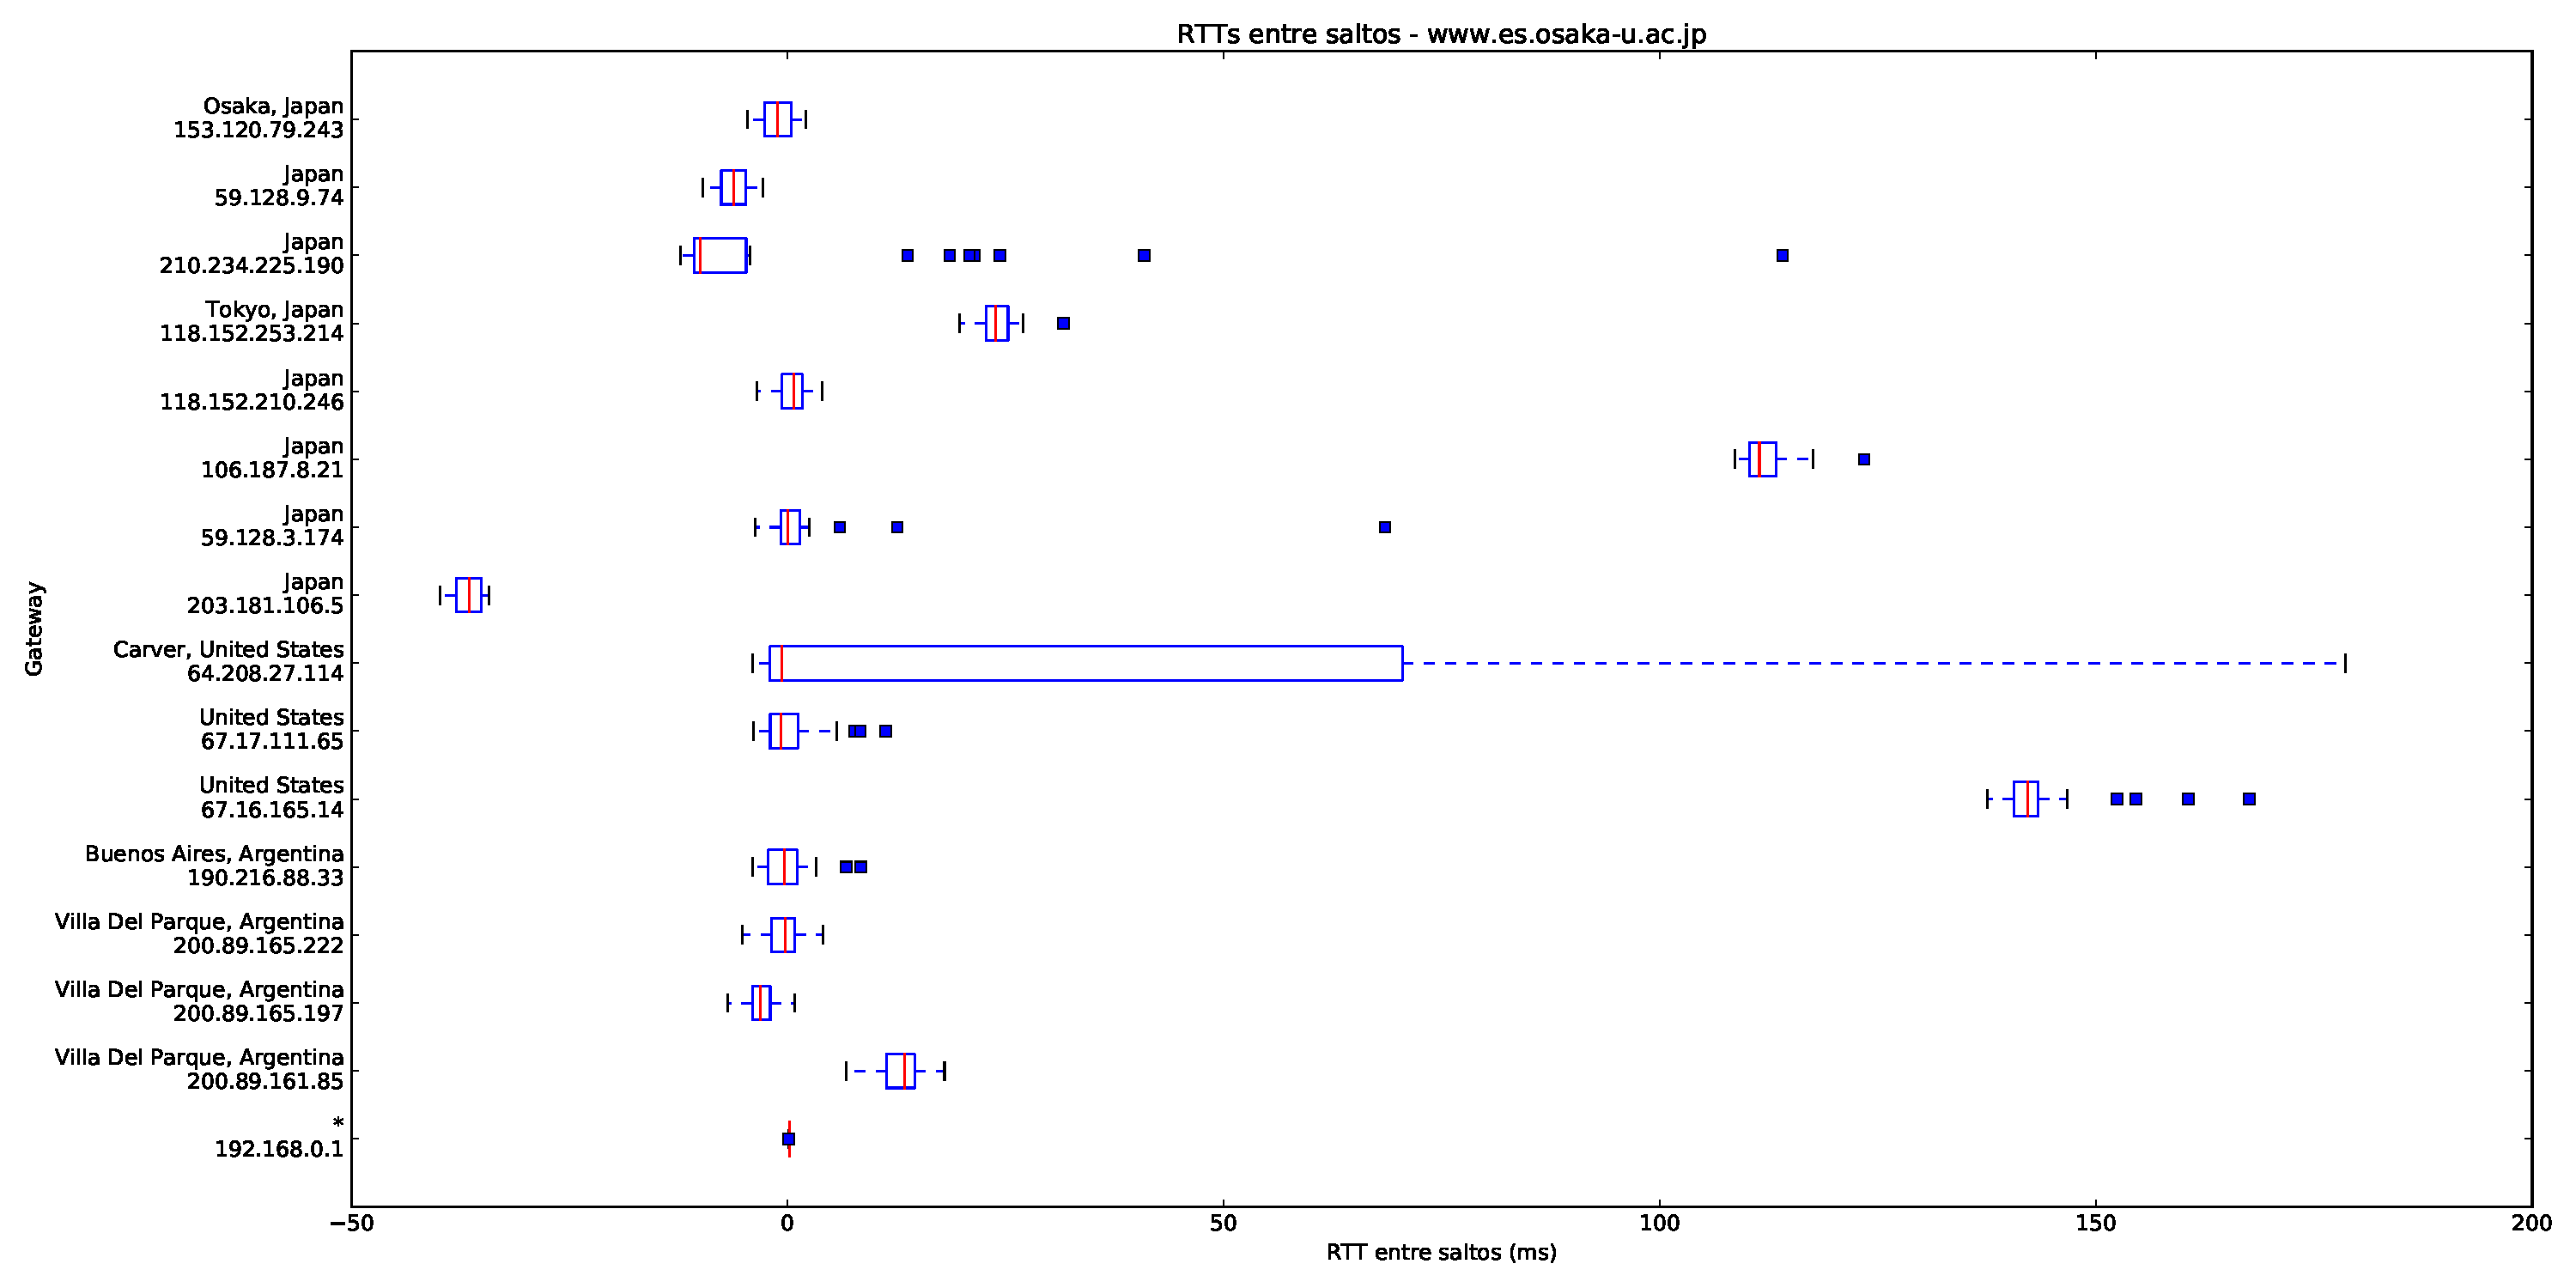
\includegraphics[width=8.5cm]{img/grafico1-www-es-osaka-u-ac-jp.pdf}
    \caption{\normalfont RTTs entre saltos. El valor asignado al $i$-ésimo nodo corresponde al salto entre el $i$-ésimo y el $i - 1$-ésimo nodo. Para el primer nodo se utiliza simplemente su RTT.}
\end{figure}

\begin{figure}[H]
    \centering
    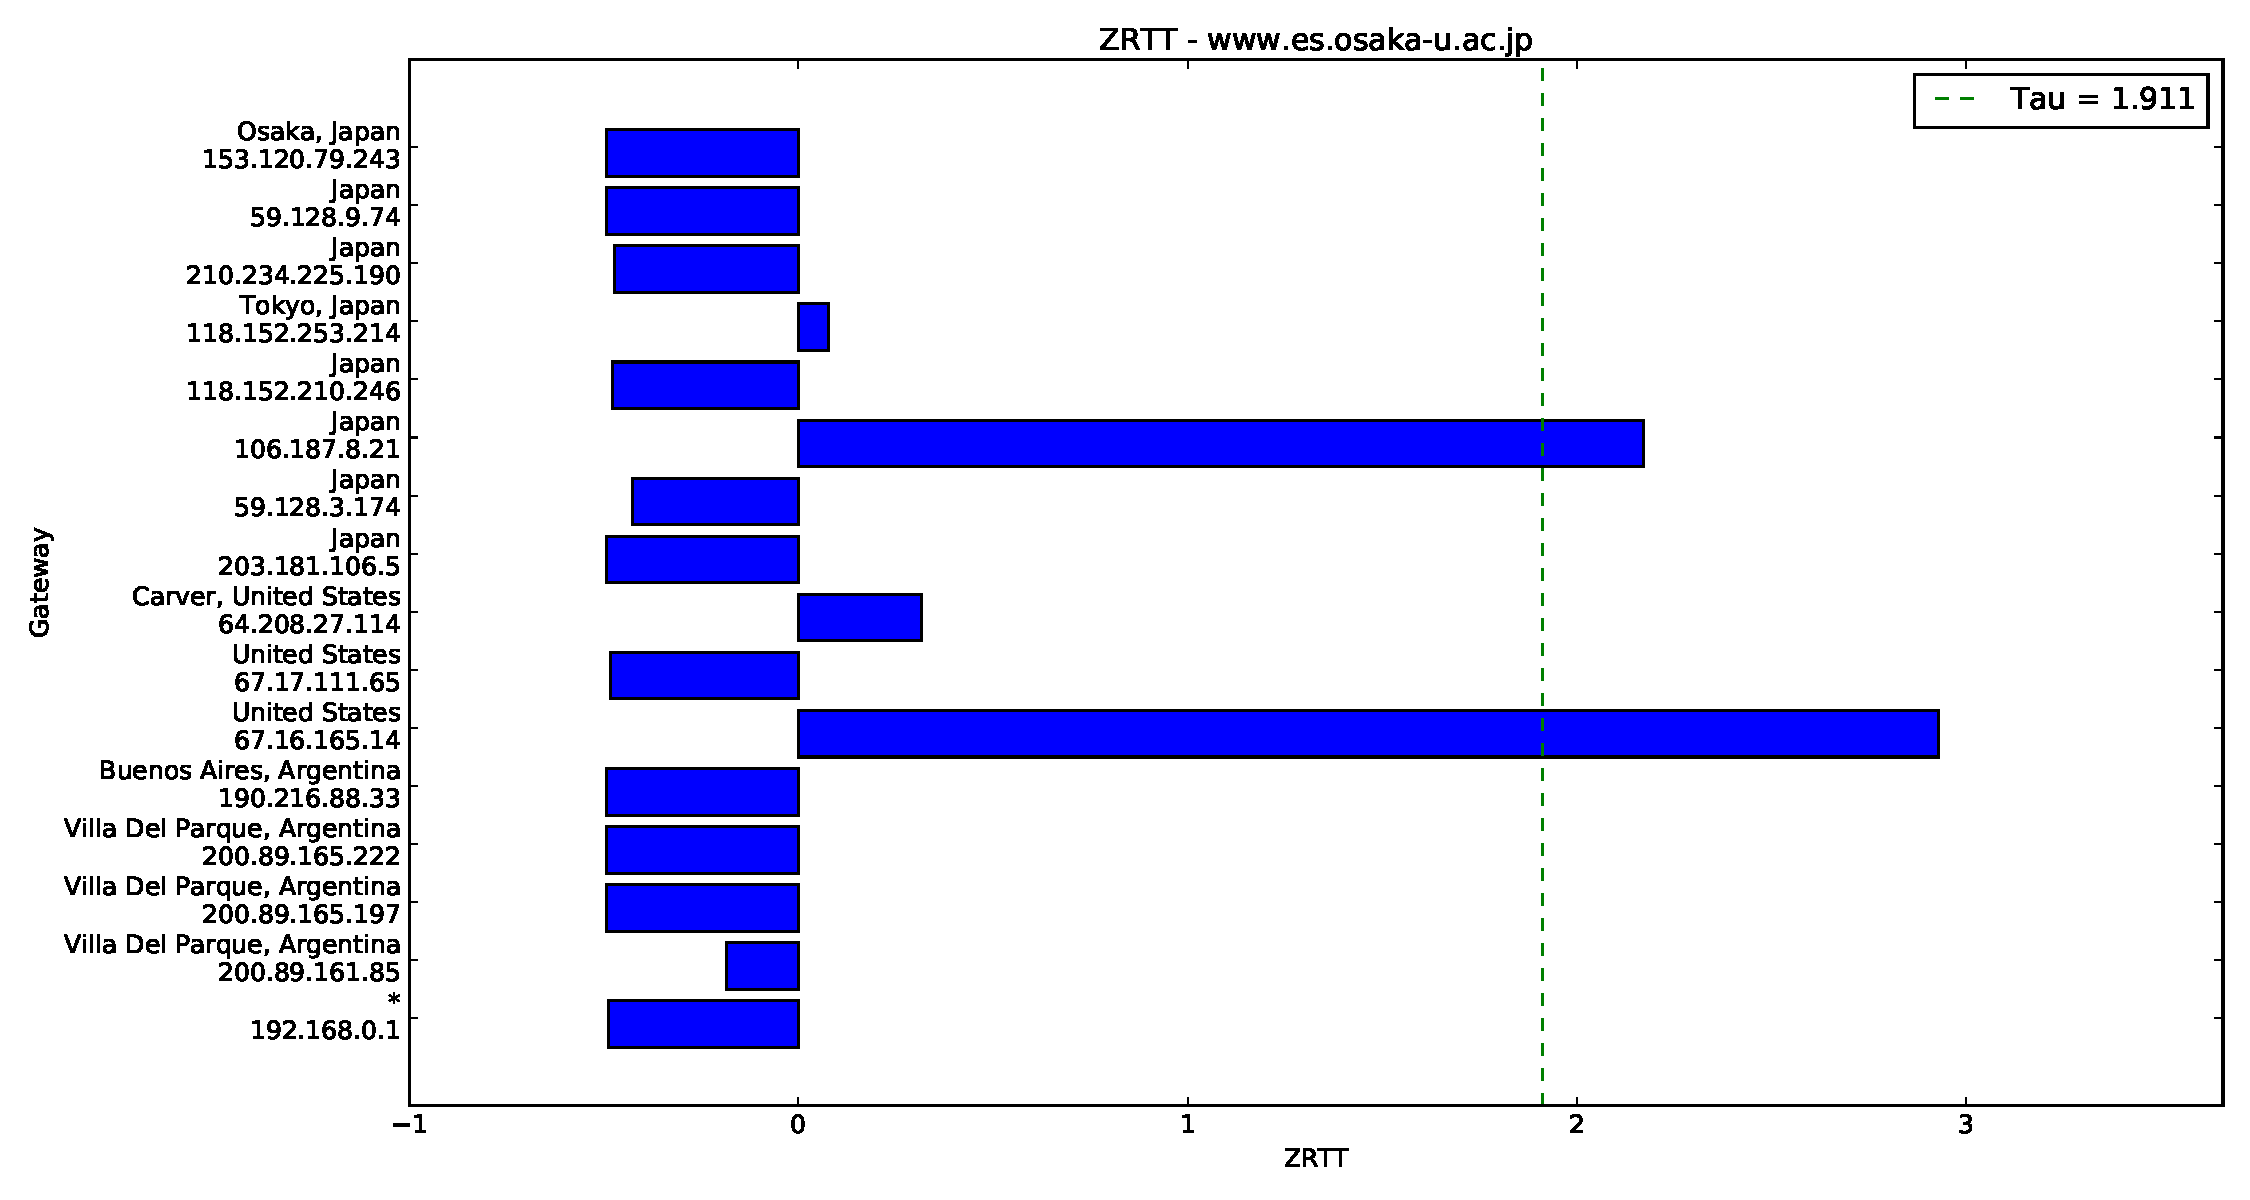
\includegraphics[width=8.5cm]{img/grafico2-www-es-osaka-u-ac-jp.pdf}
    \caption{\normalfont ZRTTs entre saltos.}
\end{figure}

Sin embargo, en el gráfico de $ZRTT$ podemos observar problemas con la geolocalización IP. Hay 2 IPs en la ruta que nos indican que el gateway está en Japón, pero recién el tercero está indicado como un enlace intercontinental.
Esto nos permite afirmar, con bastante seguridad, que las dos primeras IP que según el servicio de geolocalización IP están en Japón (\texttt{203.181.106.5} y \texttt{59.128.3.174}), están en realidad en Estados Unidos.

El porcentaje de saltos que no responden los time exceeded es 30.43\% (exactamente 7 de 23). En términos de saltos que sí responden, la ruta tiene 16 nodos, incluyendo nuestro router.

\begin{figure}[H]
    \centering
    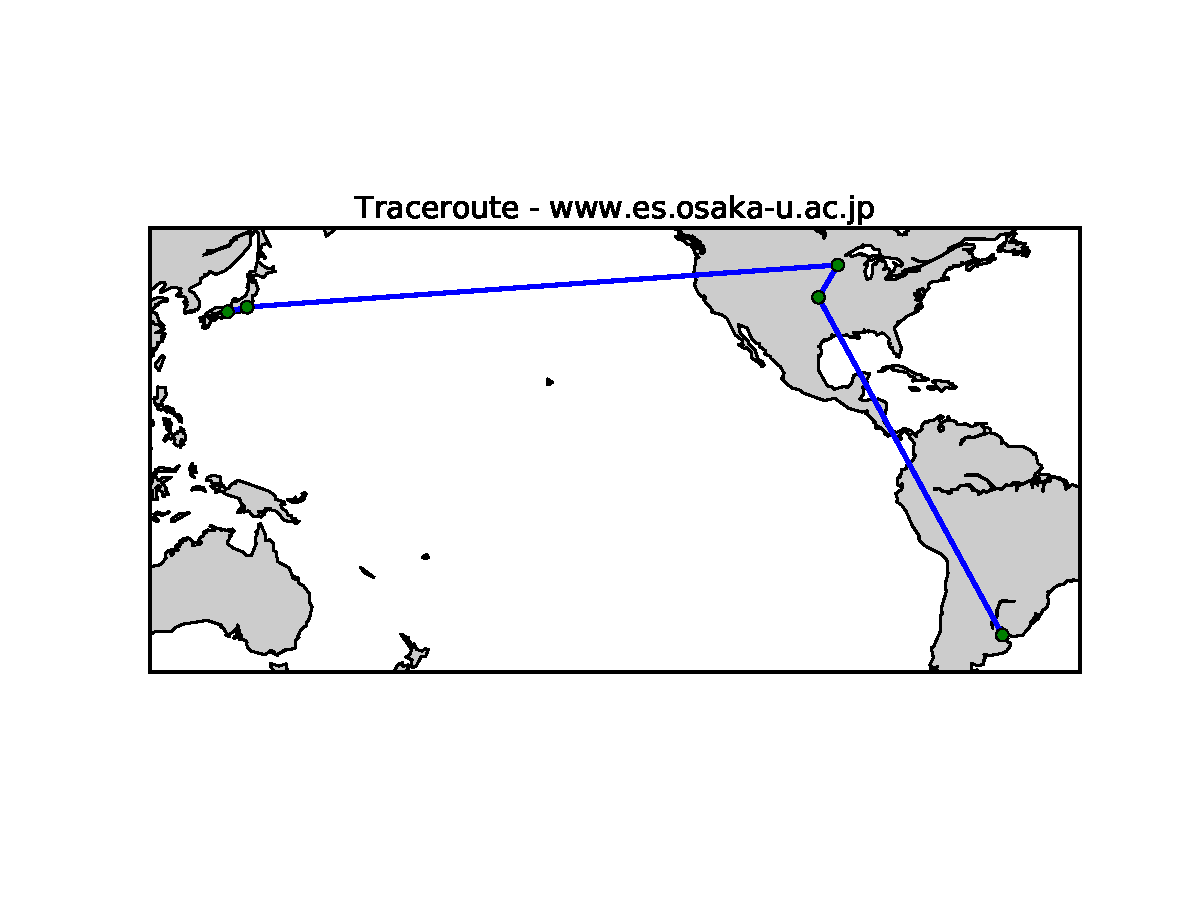
\includegraphics[width=8.5cm]{img/grafico3-www-es-osaka-u-ac-jp.pdf}
    \caption{\normalfont Ubicación geográfica estimada de la ruta tomada.}
\end{figure}


Como se ve, la ruta es aproximadamente la esperada. La ruta como bien se observa en el mapa, tiene 2 saltos intercontinentales, y como bien predijo nuestro modelo, tiene 2 enlaces submarinos, uno entre Argentina y Estados Unidos, y otro entre Estados Unidos y Japón.

En este caso el modelo fue extremadamente preciso: hay 2 enlaces submarinos y nuestro modelo los detectó, y no detectó ninguno más (es decir, no hubo falsos negativos).





\subsection{Université de Laval}

A continuación presentamos los gráficos resultantes de realizar una \textit{traceroute} a la página de la Université de Laval\footnote{www2.ulaval.ca.}.

\begin{figure}[H]
    \centering
    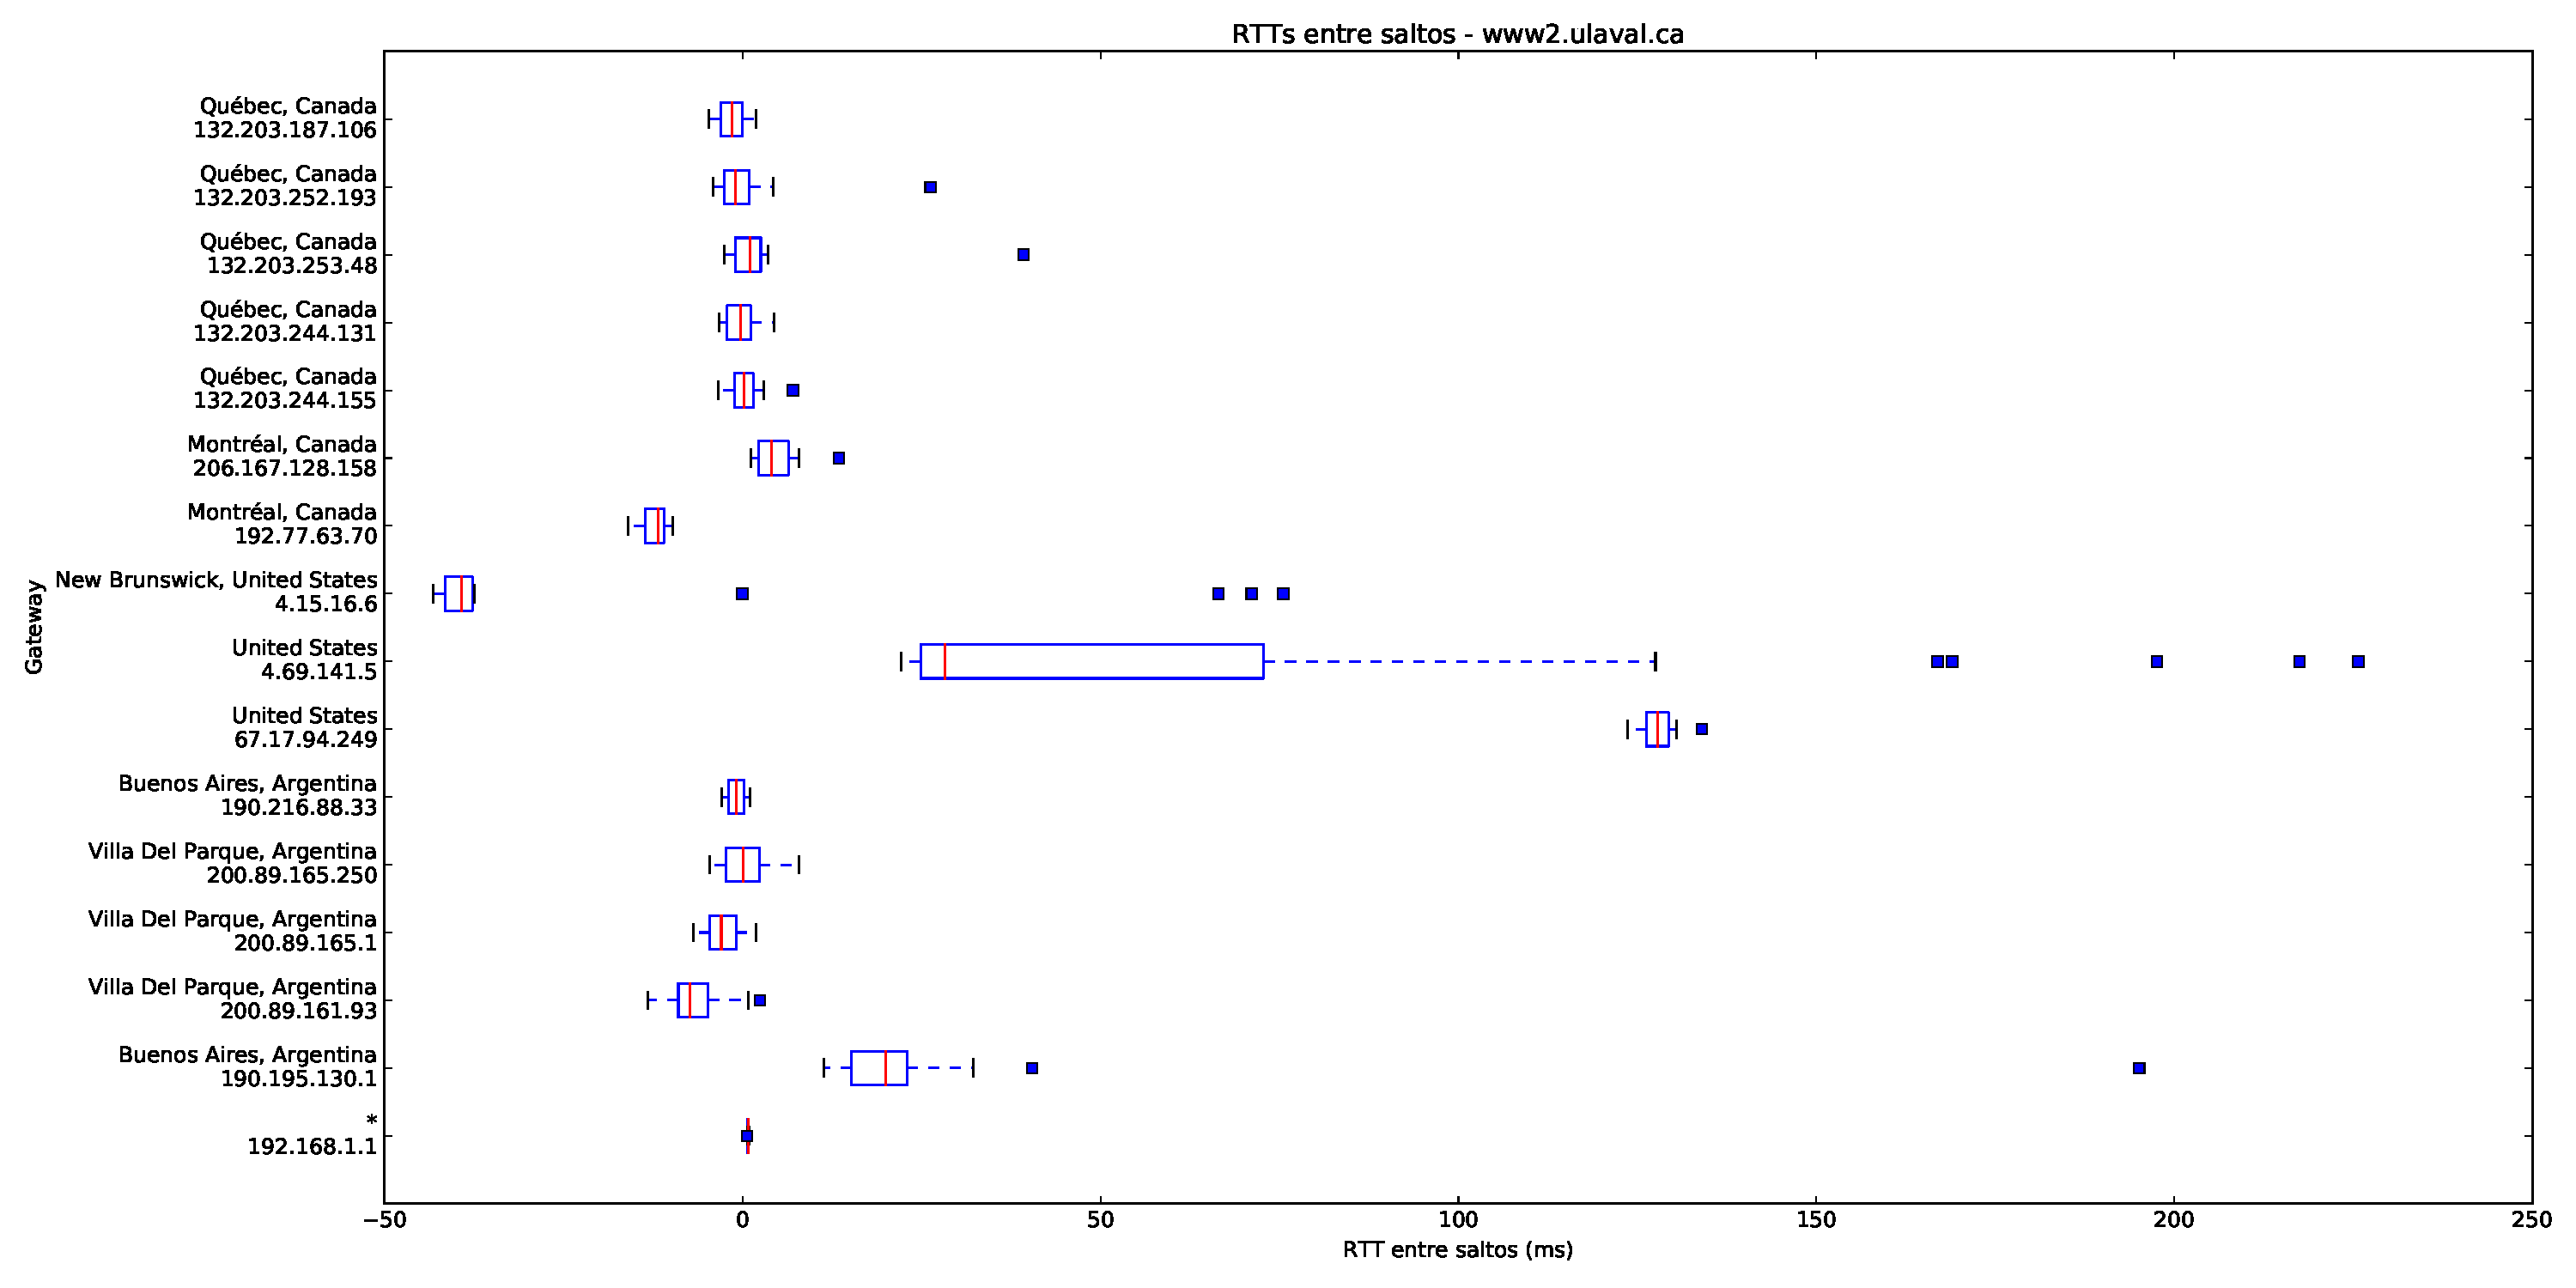
\includegraphics[width=8.5cm]{img/grafico1-www2-ulaval-ca.pdf}
    \caption{\normalfont RTTs entre saltos. El valor asignado al $i$-ésimo nodo corresponde al salto entre el $i$-ésimo y el $i - 1$-ésimo nodo. Para el primer nodo se utiliza simplemente su RTT.}
    \label{graf1L}
\end{figure}

\par En la realización de la \textit{traceroute}, 6 de los 22 ($27.\overline{27}\%$) nodos no respondieron los \textit{Time exceeded}.

\par Observamos una cantidad de \textit{outliers} y una desviación consistente entre los distintos saltos en la figura \ref{graf1L}.
Esto posiblemente se debe a una congestión momentárea en la red durante ciertas repticiones de la \textit{traceroute}, resultanto en que todos los RTTs de la repetición sean considerados \textit{outliers}.

\par Si bien la mayoría de los nodos presentan desviaciones similares, en el de dirección 4.69.141.5 se observa una varianza excepcionalmente alta.
Esto se puede deber a algunos de los factores mencionados en Jobst 2012\cite{anomalias}: métodos de balanceo de carga variando las rutas de los paquetes de diversas mediciones, o caminos de ida/vuelta asimétricos resultando en RTTs inconsistentes.

\begin{figure}[H]
    \centering
    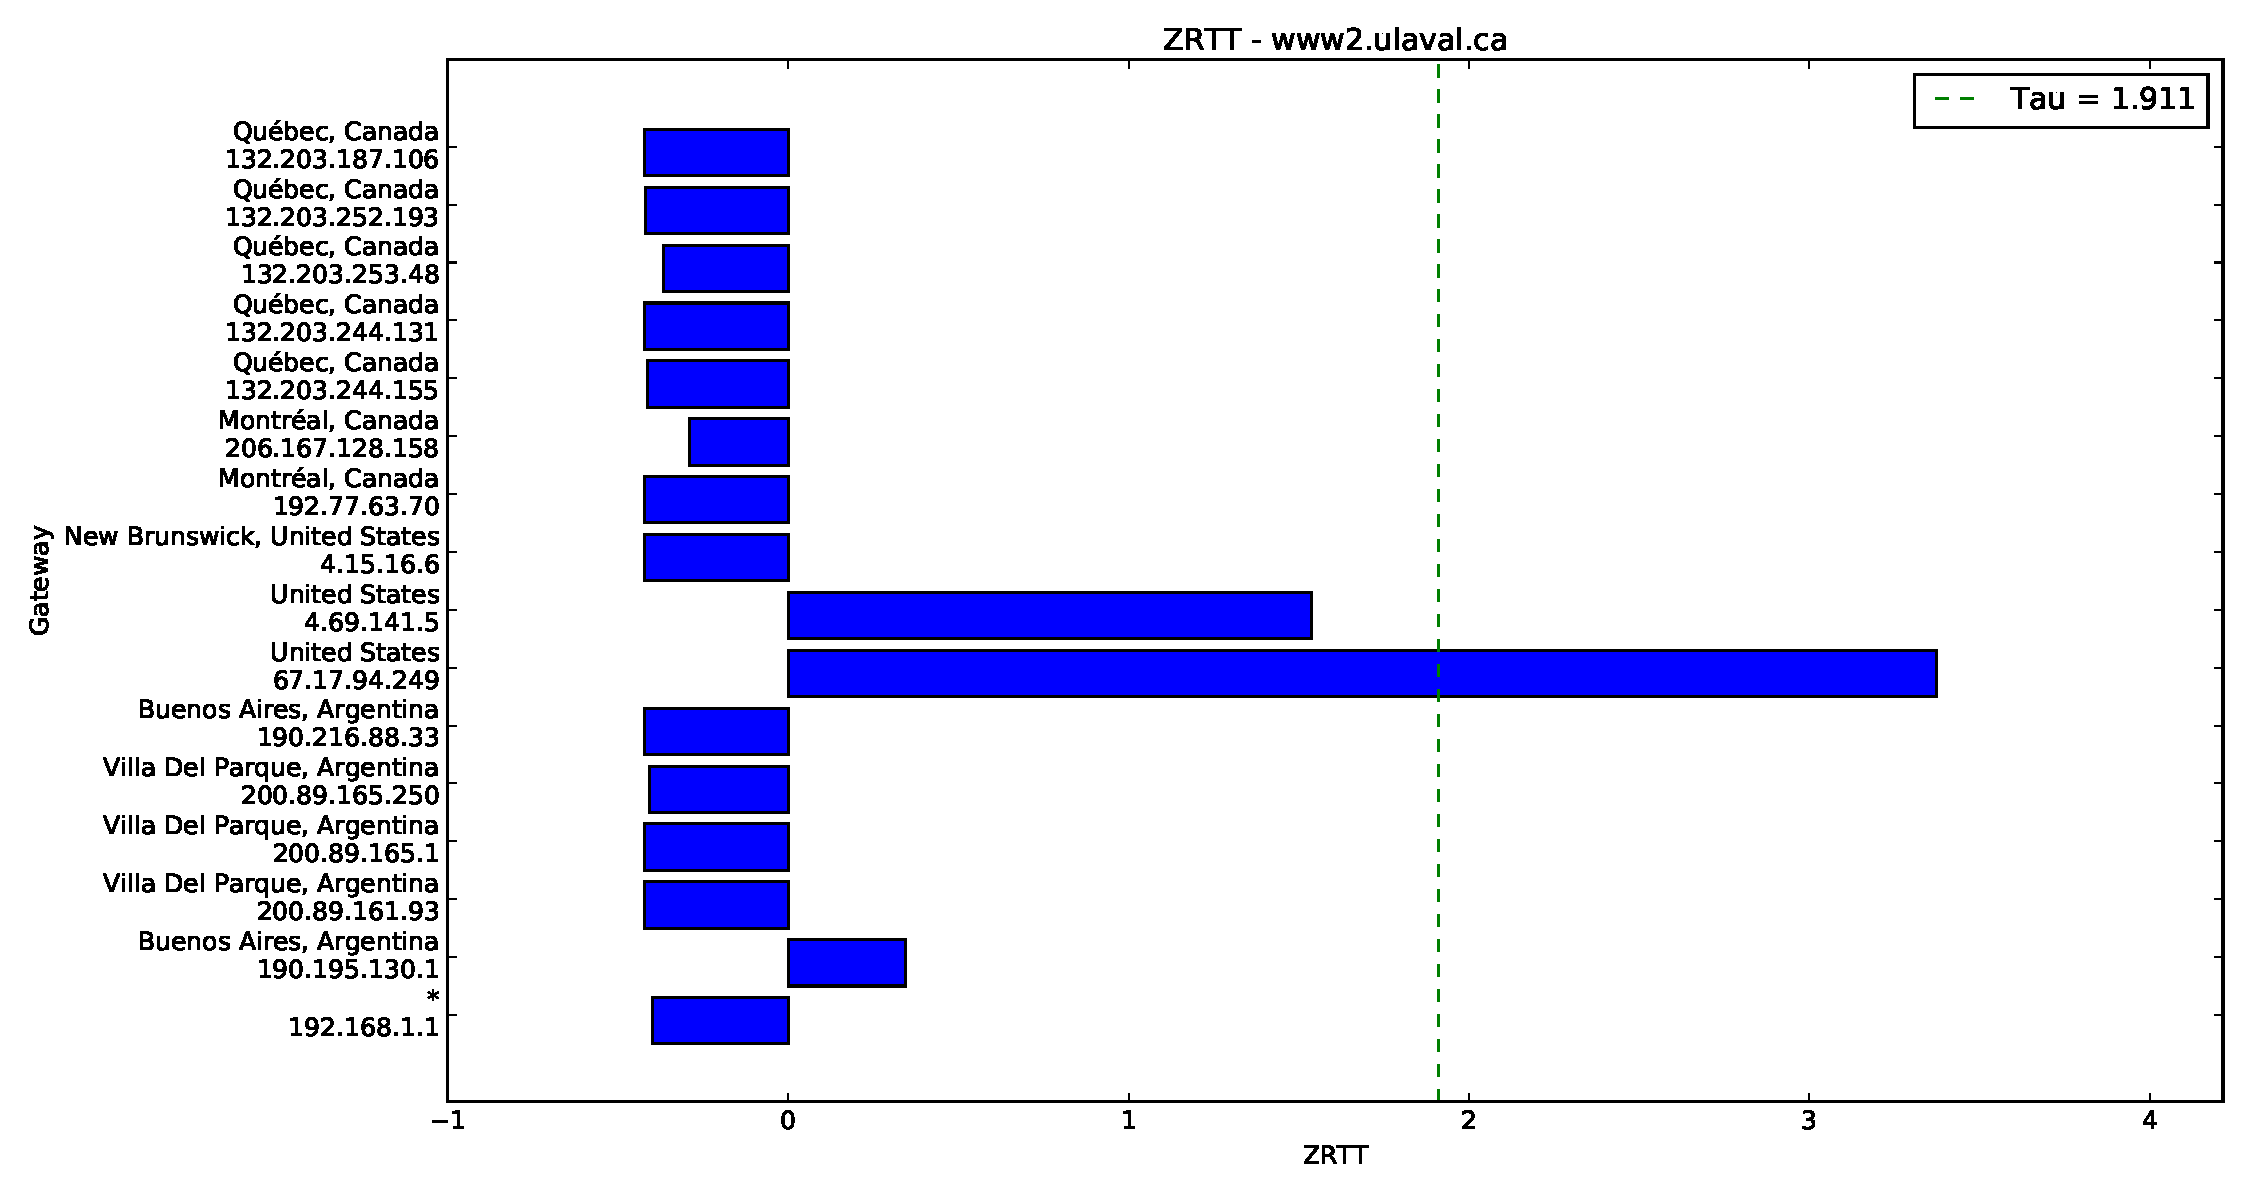
\includegraphics[width=8.5cm]{img/grafico2-www2-ulaval-ca.pdf}
    \caption{\normalfont ZRTTs entre saltos.}
\end{figure}

\begin{figure}[H]
    \centering
    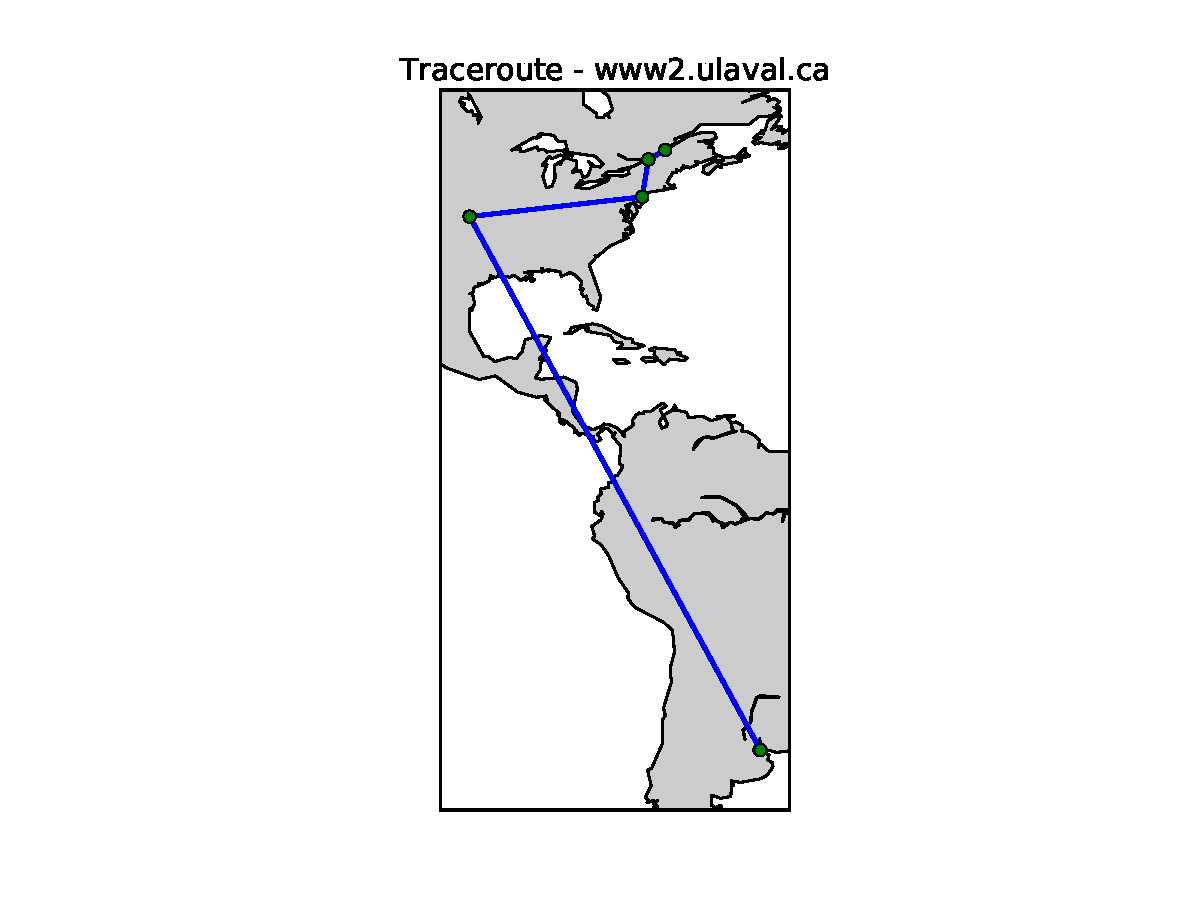
\includegraphics[width=8.5cm]{img/grafico3-www2-ulaval-ca.pdf}
    \caption{\normalfont Ubicación geográfica estimada de la ruta tomada.}
    \label{mapaLaval}
\end{figure}

\par Sólo un salto (de 200.89.165.250 a 67.17.94.249) se presentó como \textit{outlier} según el método planteado\cite{outliers}.
De acuerdo a la estimación geográfica, este salto se da entre Buenos Aires y Estados Unidos.

\par No hay ningún cable submarino que una directamente a Argentina con Estados Unidos.
Sin embargo se pueden trazar rutas submarinas componiendo distintos cables submarinos entre ambos extremos\footnote{Por ejemplo, el South American Crossing (SAC) une a Argentina con Panamá y el Pan-American Crossing (PAC) a Panamá con Estados Unidos.}.

\par Si bien estos dos hechos parecen contradecirse, Jobst 2012\cite{anomalias} provee una explicación: routers de \textit{MPLS}\footnote{\textit{Multiprotocol Label Switching (MPLS)} es un protocolo empleado para simplificar el \textit{forwarding}.} que no honran el campo \textit{TTL}, y por ende no aparecen en la \textit{traceroute}.
Los cables submarinos manejan un flujo muy alto de paquetes, por lo que es esperable que busquen optimizar la performance; ignorar el campo \textit{TTL} es una forma de logarlo.
Esto resulta en que toda la ruta entre Buenos Aires y Estados Unidos se vea condensada en un único salto.

\par Cabe destacar que la herramienta geógrafica utilizada no pudo proveer la latitud y longitud de la dirección IP 67.17.94.249, por lo que el mapa emplea la próxima dirección ubicable, la 4.69.141.5.


\subsection{Universidad de Alejandría}

Presentaremos ahora los gráficos correspondientes al traceroute hacia la Universidad de Alejandría, ubicada en Alejandría, Egipto, África.

\begin{figure}[H]
    \centering
    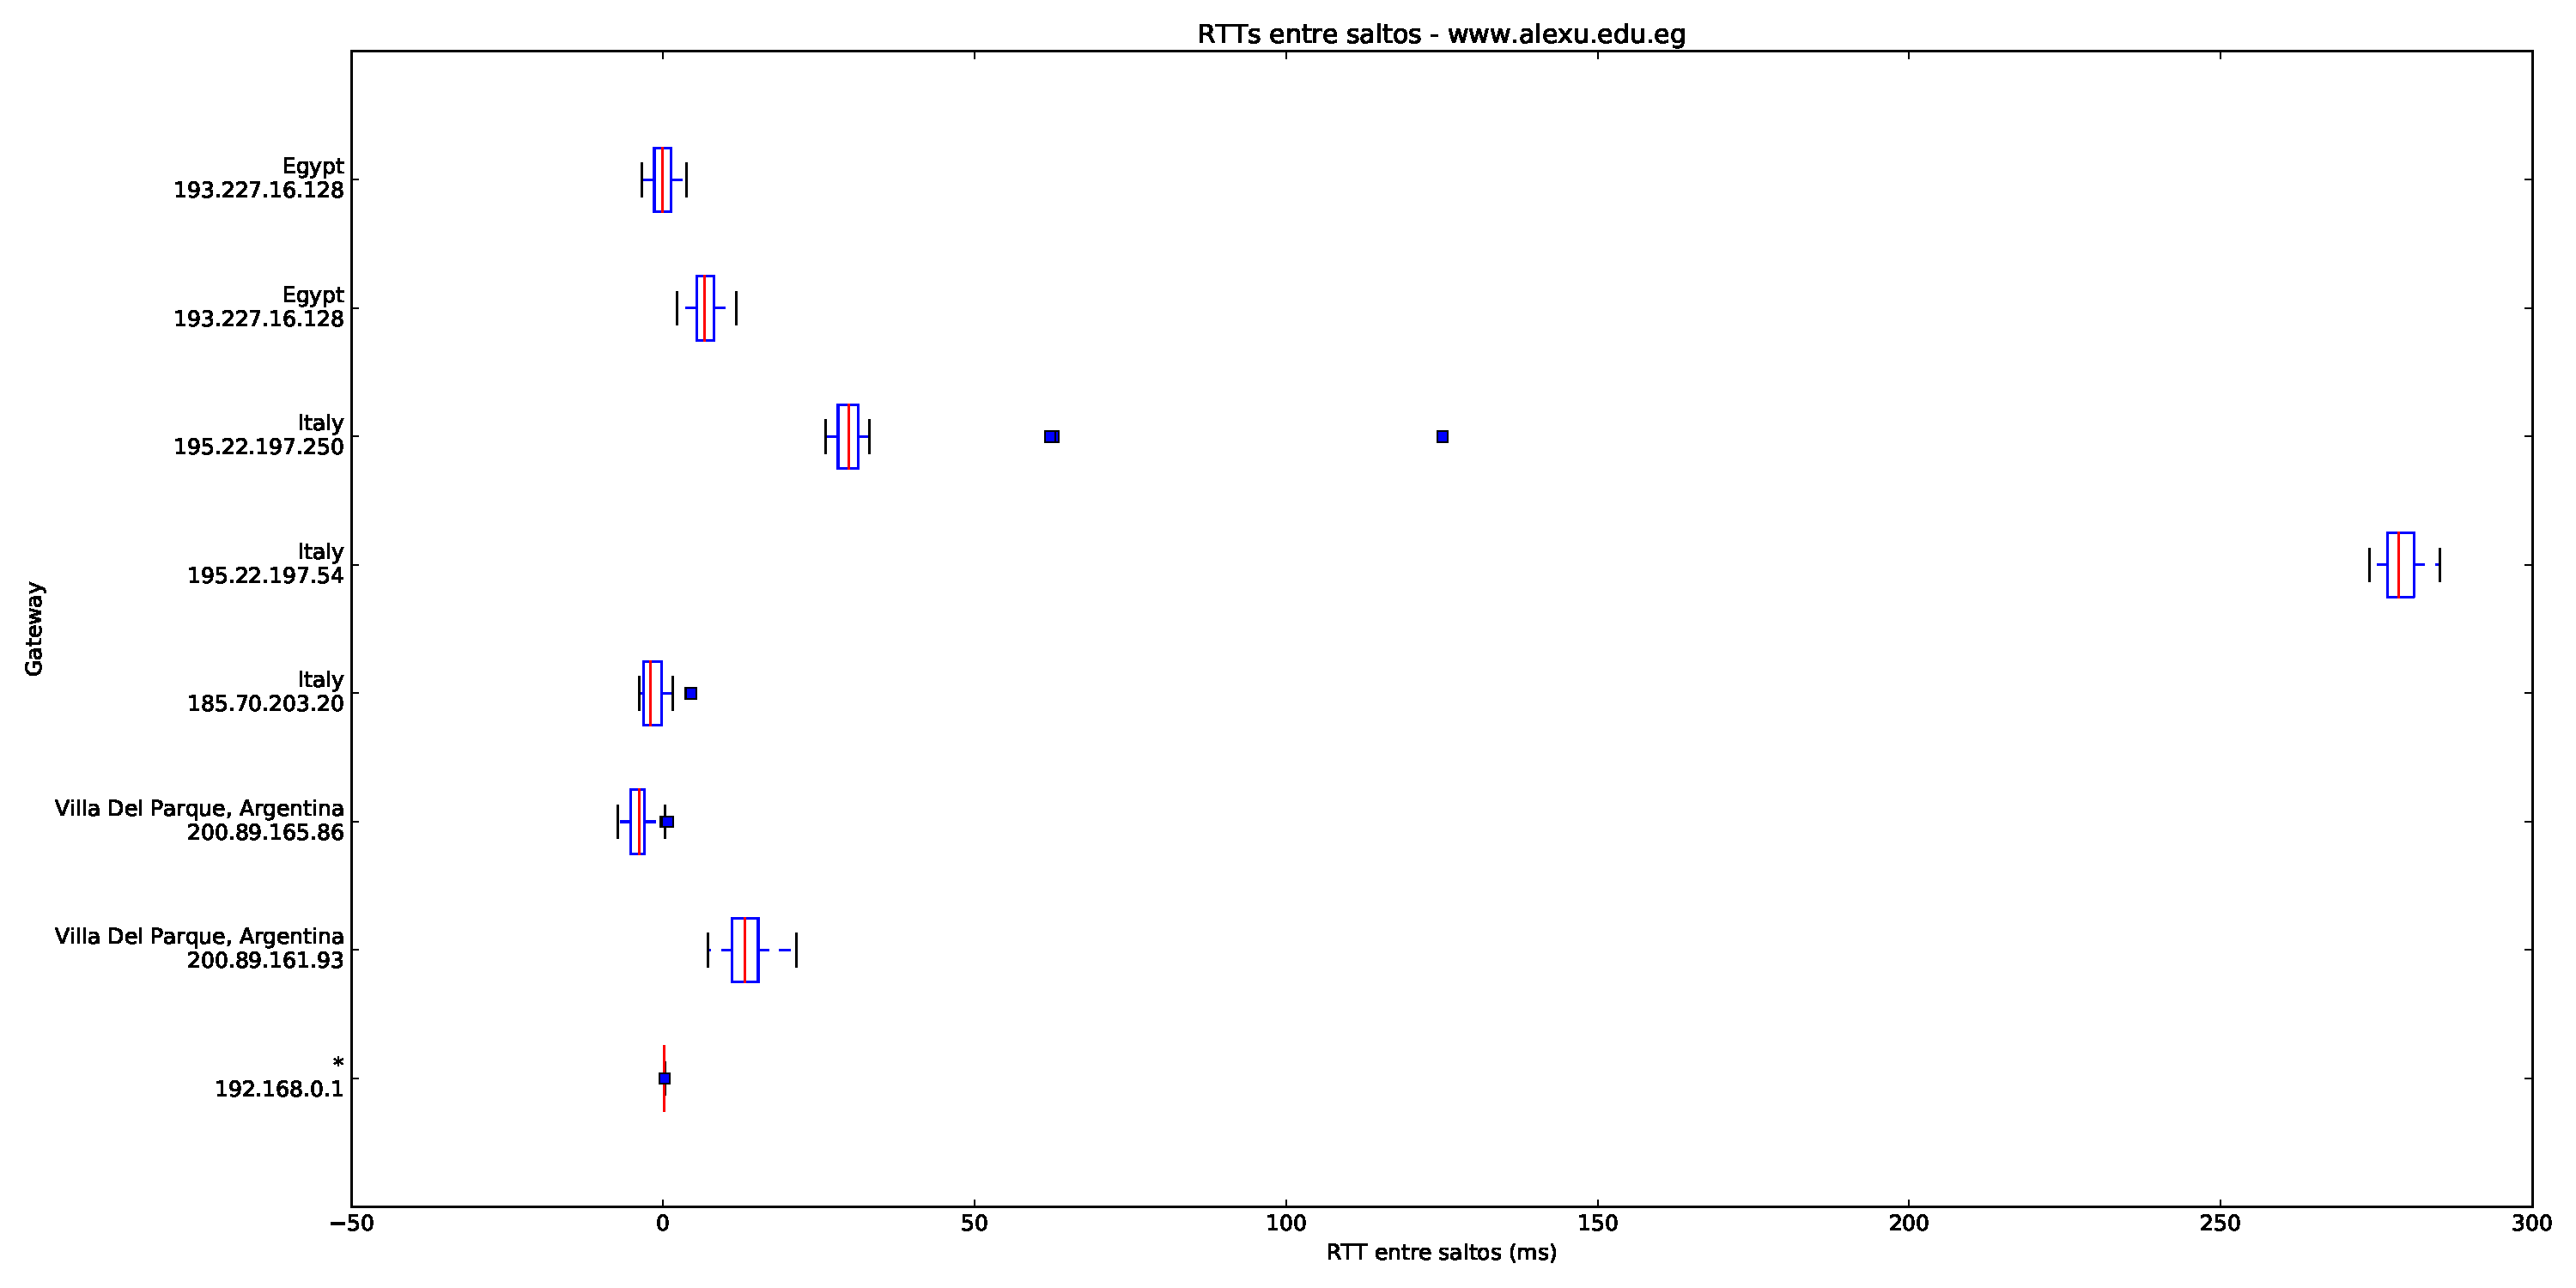
\includegraphics[width=8.5cm]{img/grafico1-www-alexu-edu-eg.pdf}
    \caption{\normalfont RTTs entre saltos. El valor asignado al $i$-ésimo nodo corresponde al salto entre el $i$-ésimo y el $i - 1$-ésimo nodo. Para el primer nodo se utiliza simplemente su RTT.}
\end{figure}

Todas las mediciones son normales en todos los gateways, y no se observan outliers. 

\begin{figure}[H]
    \centering
    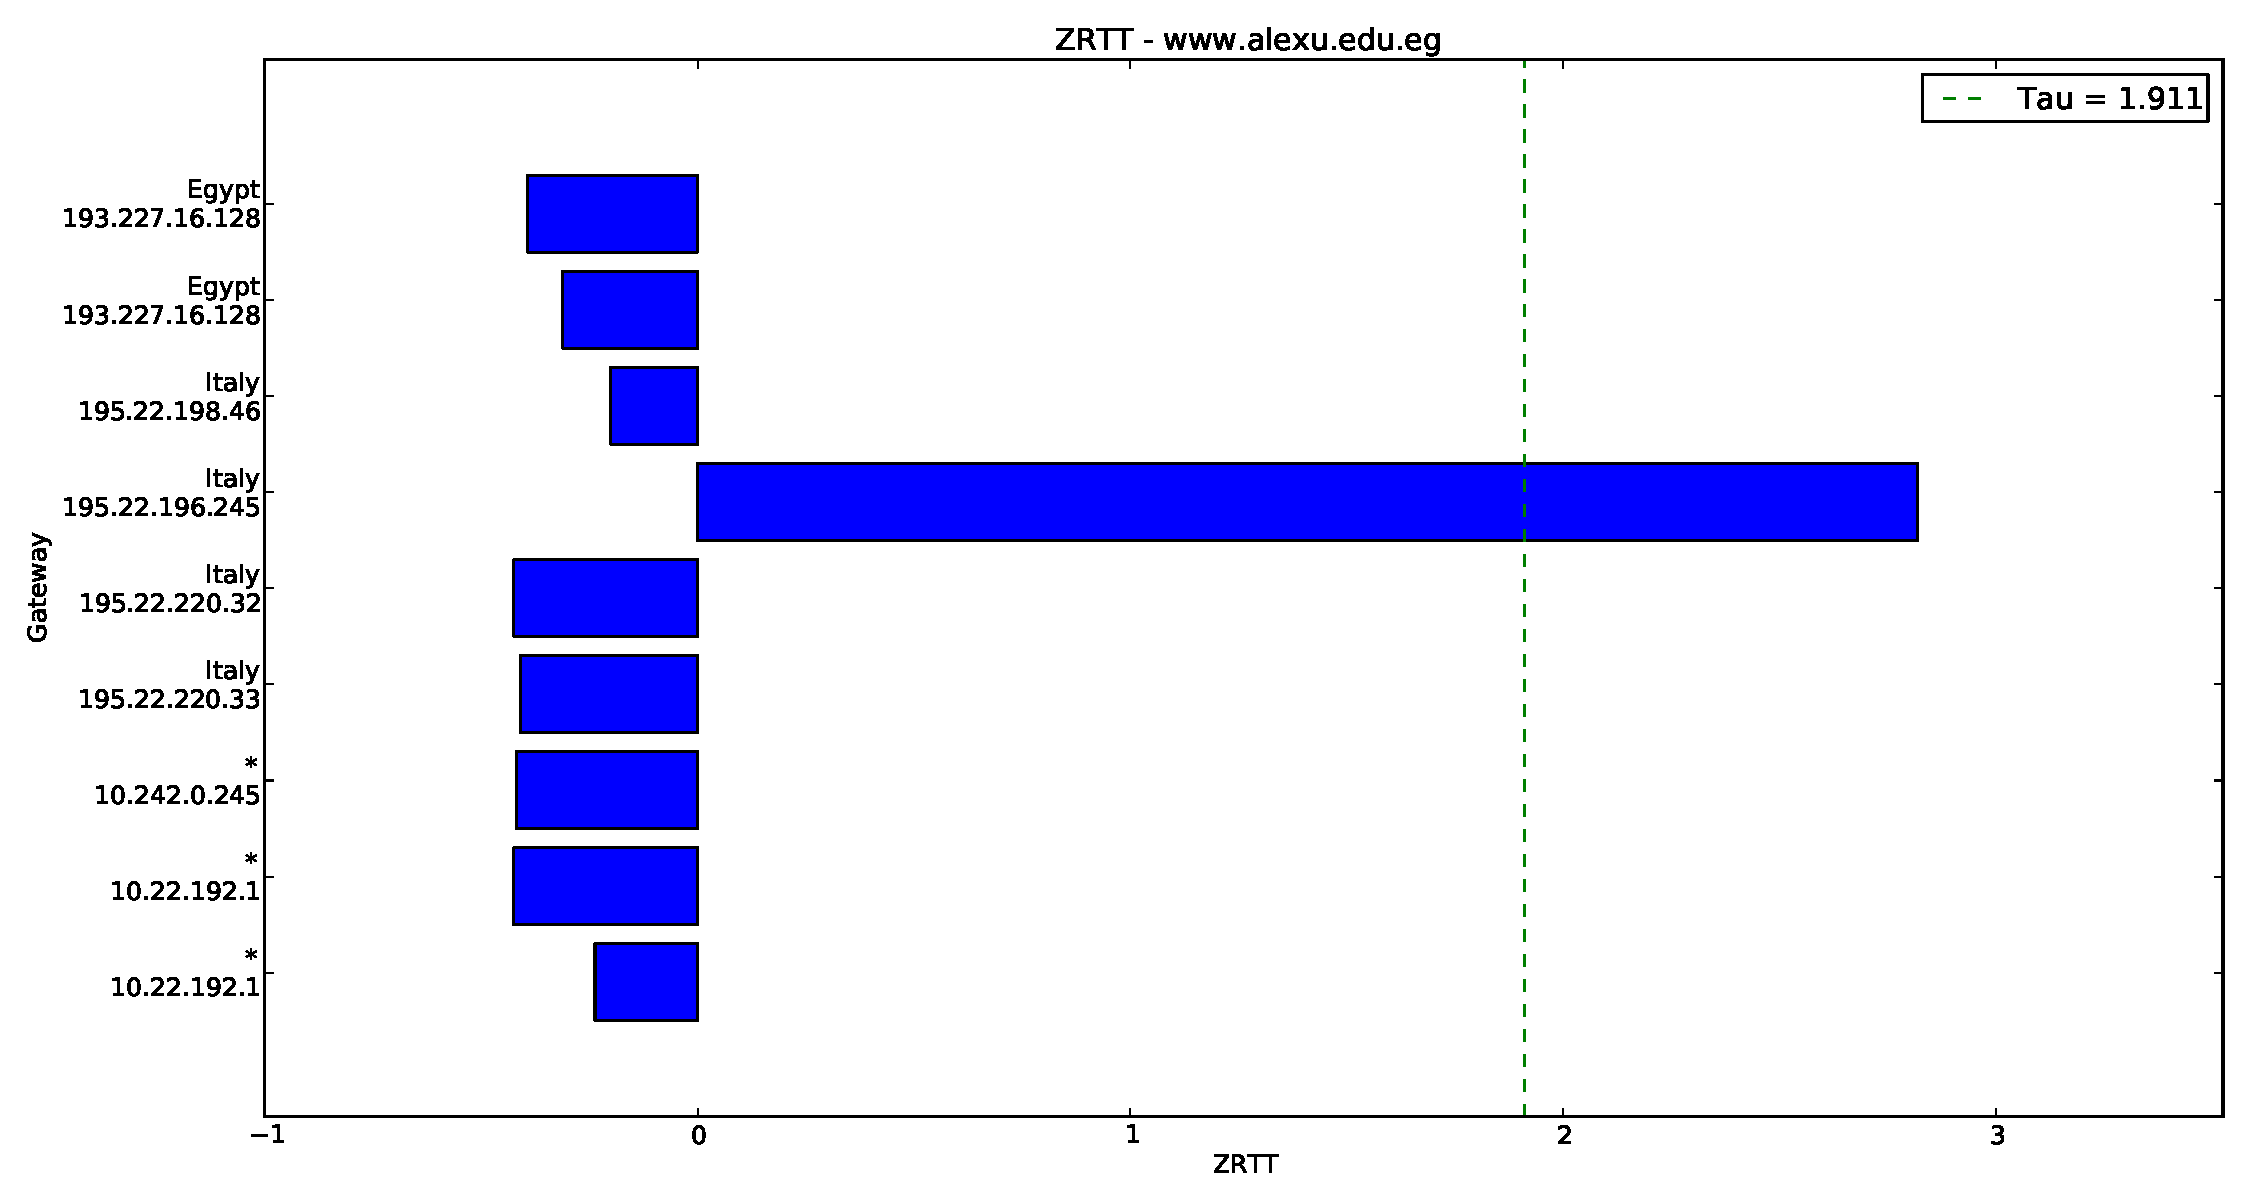
\includegraphics[width=8.5cm]{img/grafico2-www-alexu-edu-eg.pdf}
    \caption{\normalfont ZRTTs entre saltos.}
\end{figure}
En la figuta de la ruta hacia Alejandría podemos ver como tenemos problemas de geolocalización. Recién en la segunda IP que corresponde 
a Italia nos está marcando el enlace intercontinental, por lo cuál suponemos que esta primer IP italiana (185.70.203.20) en realidad
se encuentra en Argentina. 
En el traceroute, 7 de los 22 nodos no respondieron el time exceeded. 


\begin{figure}[H]
    \centering
    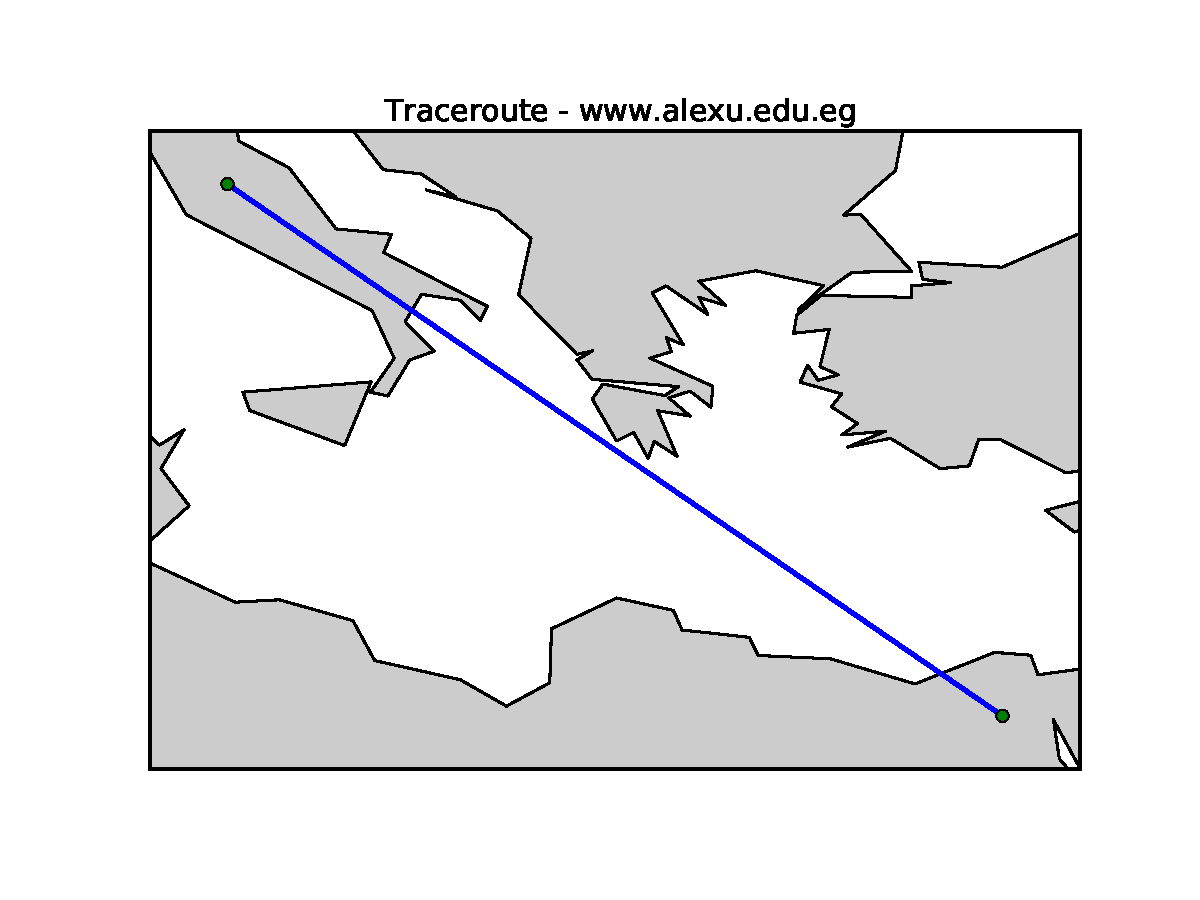
\includegraphics[width=8.5cm]{img/grafico3-www-alexu-edu-eg.pdf}
    \caption{\normalfont Ubicación geográfica estimada de la ruta tomada.}
\end{figure}

En este caso tenemos dos enlaces intercontinentales según muestra el mapa, uno de Argentina hacia Italia, y el segundo de Italia 
hacia Egipto, pero solo detectamos 1 solo enlace, el de Argentina hacia Italia, teniendo así un falso positivo. 
Esto creemos que es debido a la cercanía de Italia con Egipto, a pesar de encontrarse en países distintos. 




\subsection{Universidad de Oxford}

Este experimento corresponde a la Universidad de Oxford, ubicada en Inglaterra, cuyo dominio web es \url{www.ox.ac.uk}.

\begin{figure}[H]
    \centering
    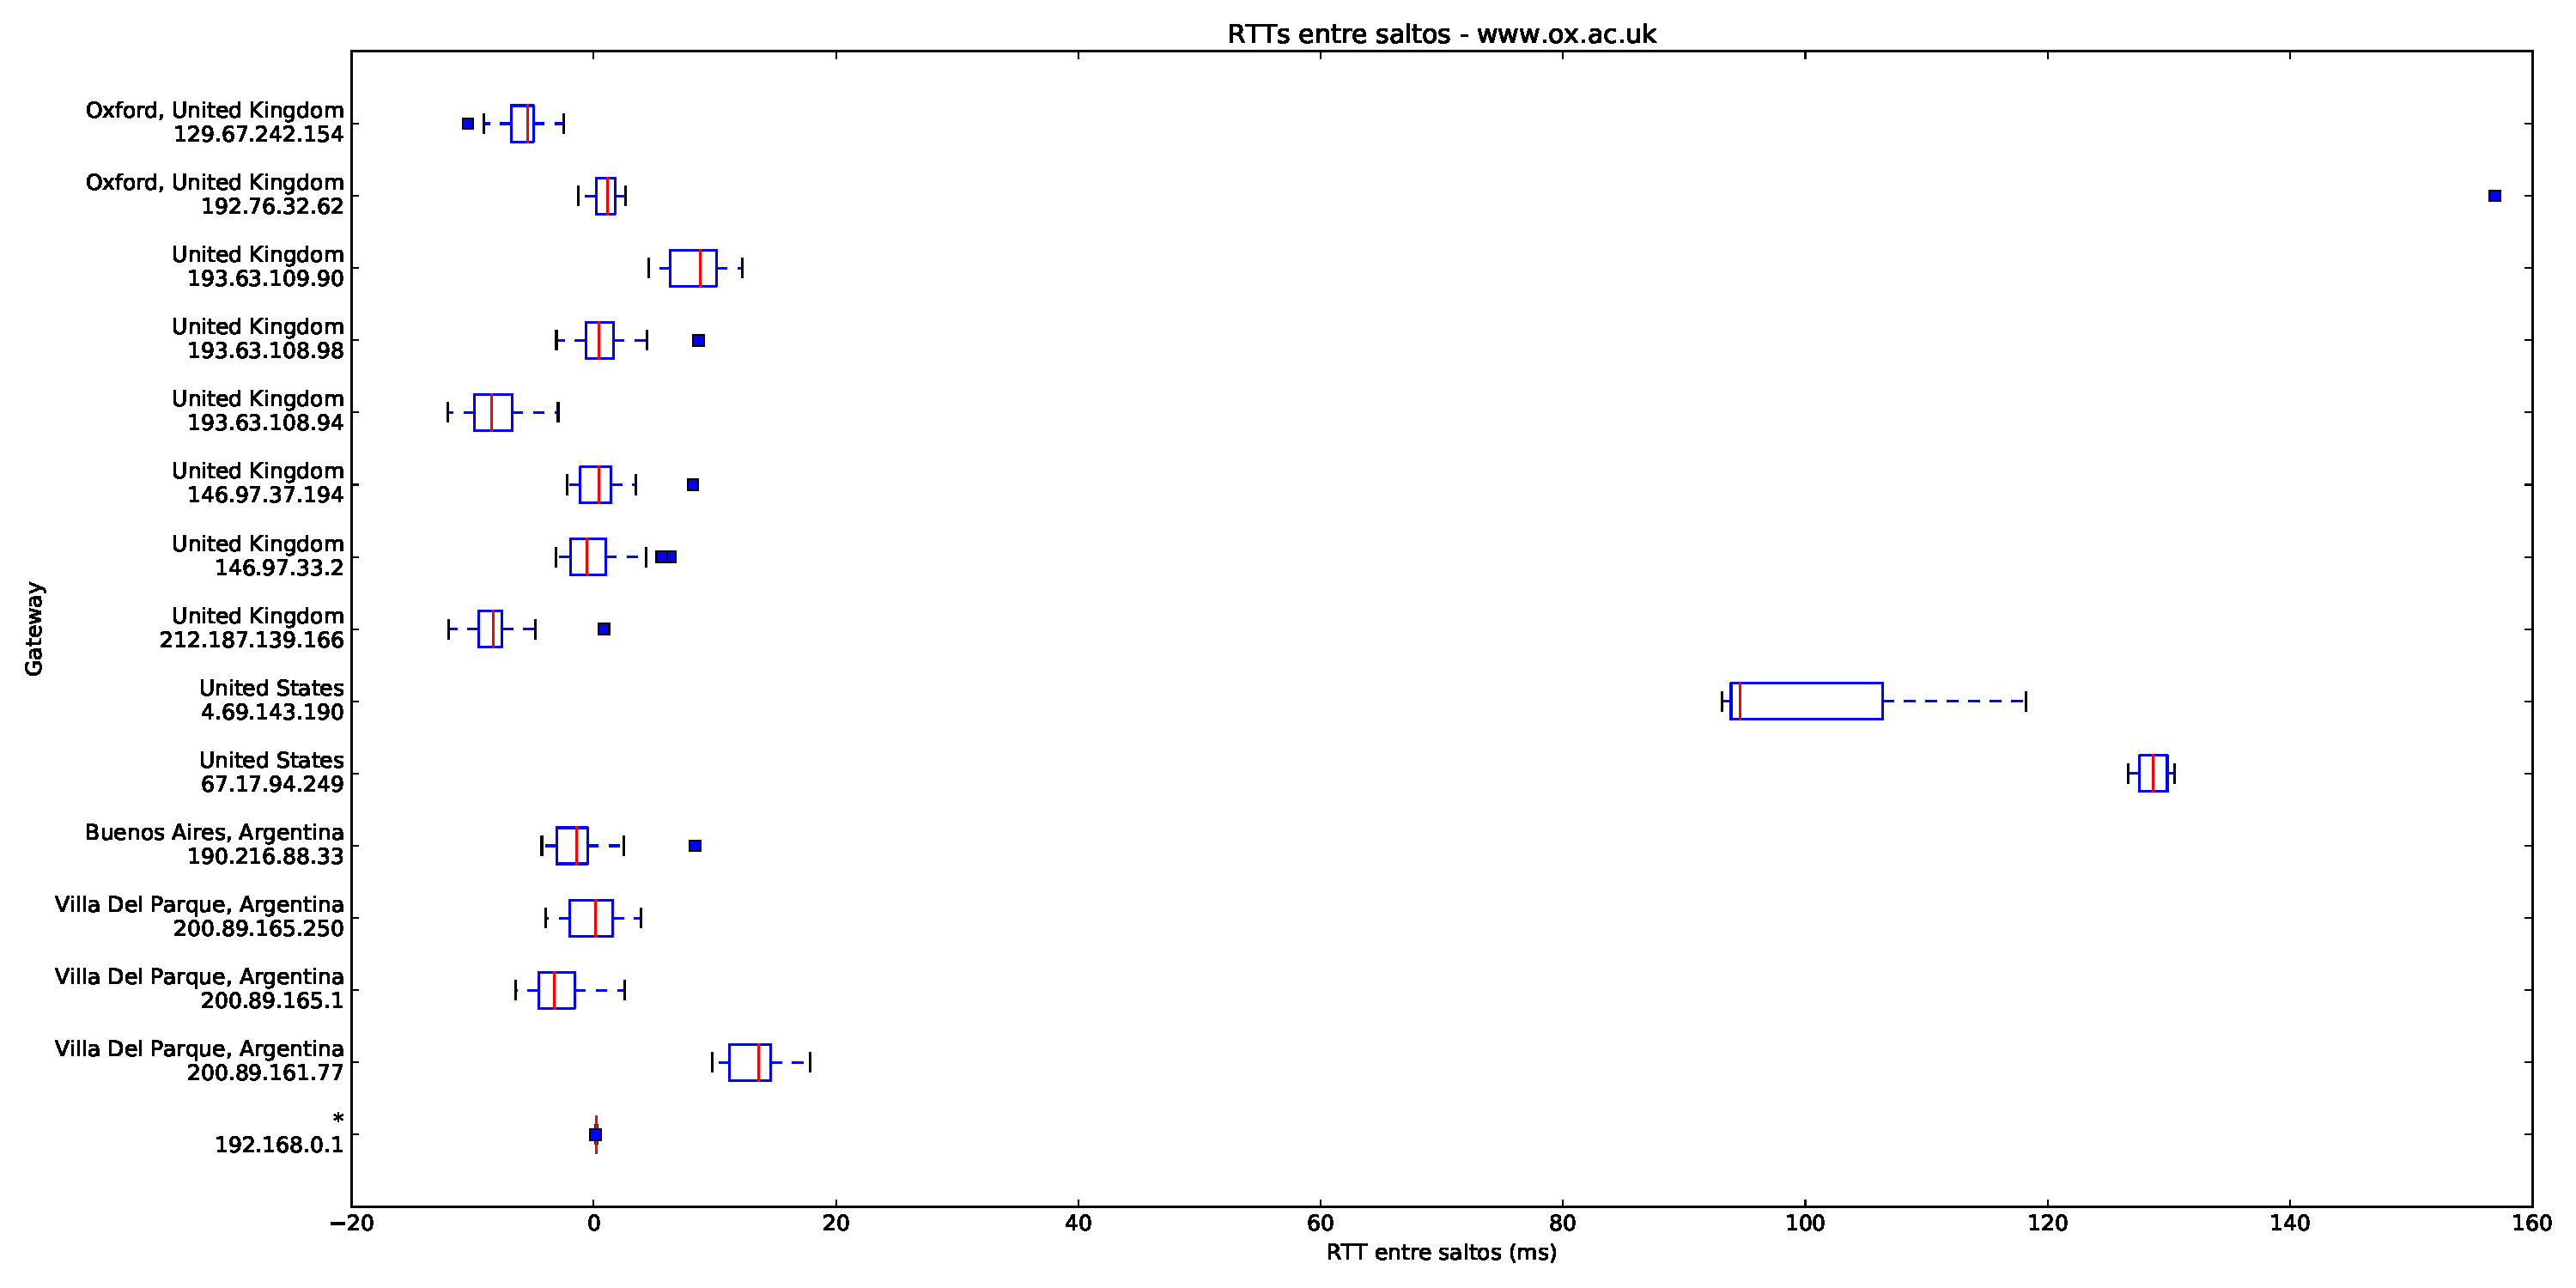
\includegraphics[width=8.5cm]{img/grafico1-www-ox-ac-uk.pdf}
    \caption{\normalfont RTTs entre saltos. El valor asignado al $i$-ésimo nodo corresponde al salto entre el $i$-ésimo y el $i - 1$-ésimo nodo. Para el primer nodo se utiliza simplemente su RTT.}
\end{figure}

\begin{figure}[H]
    \centering
    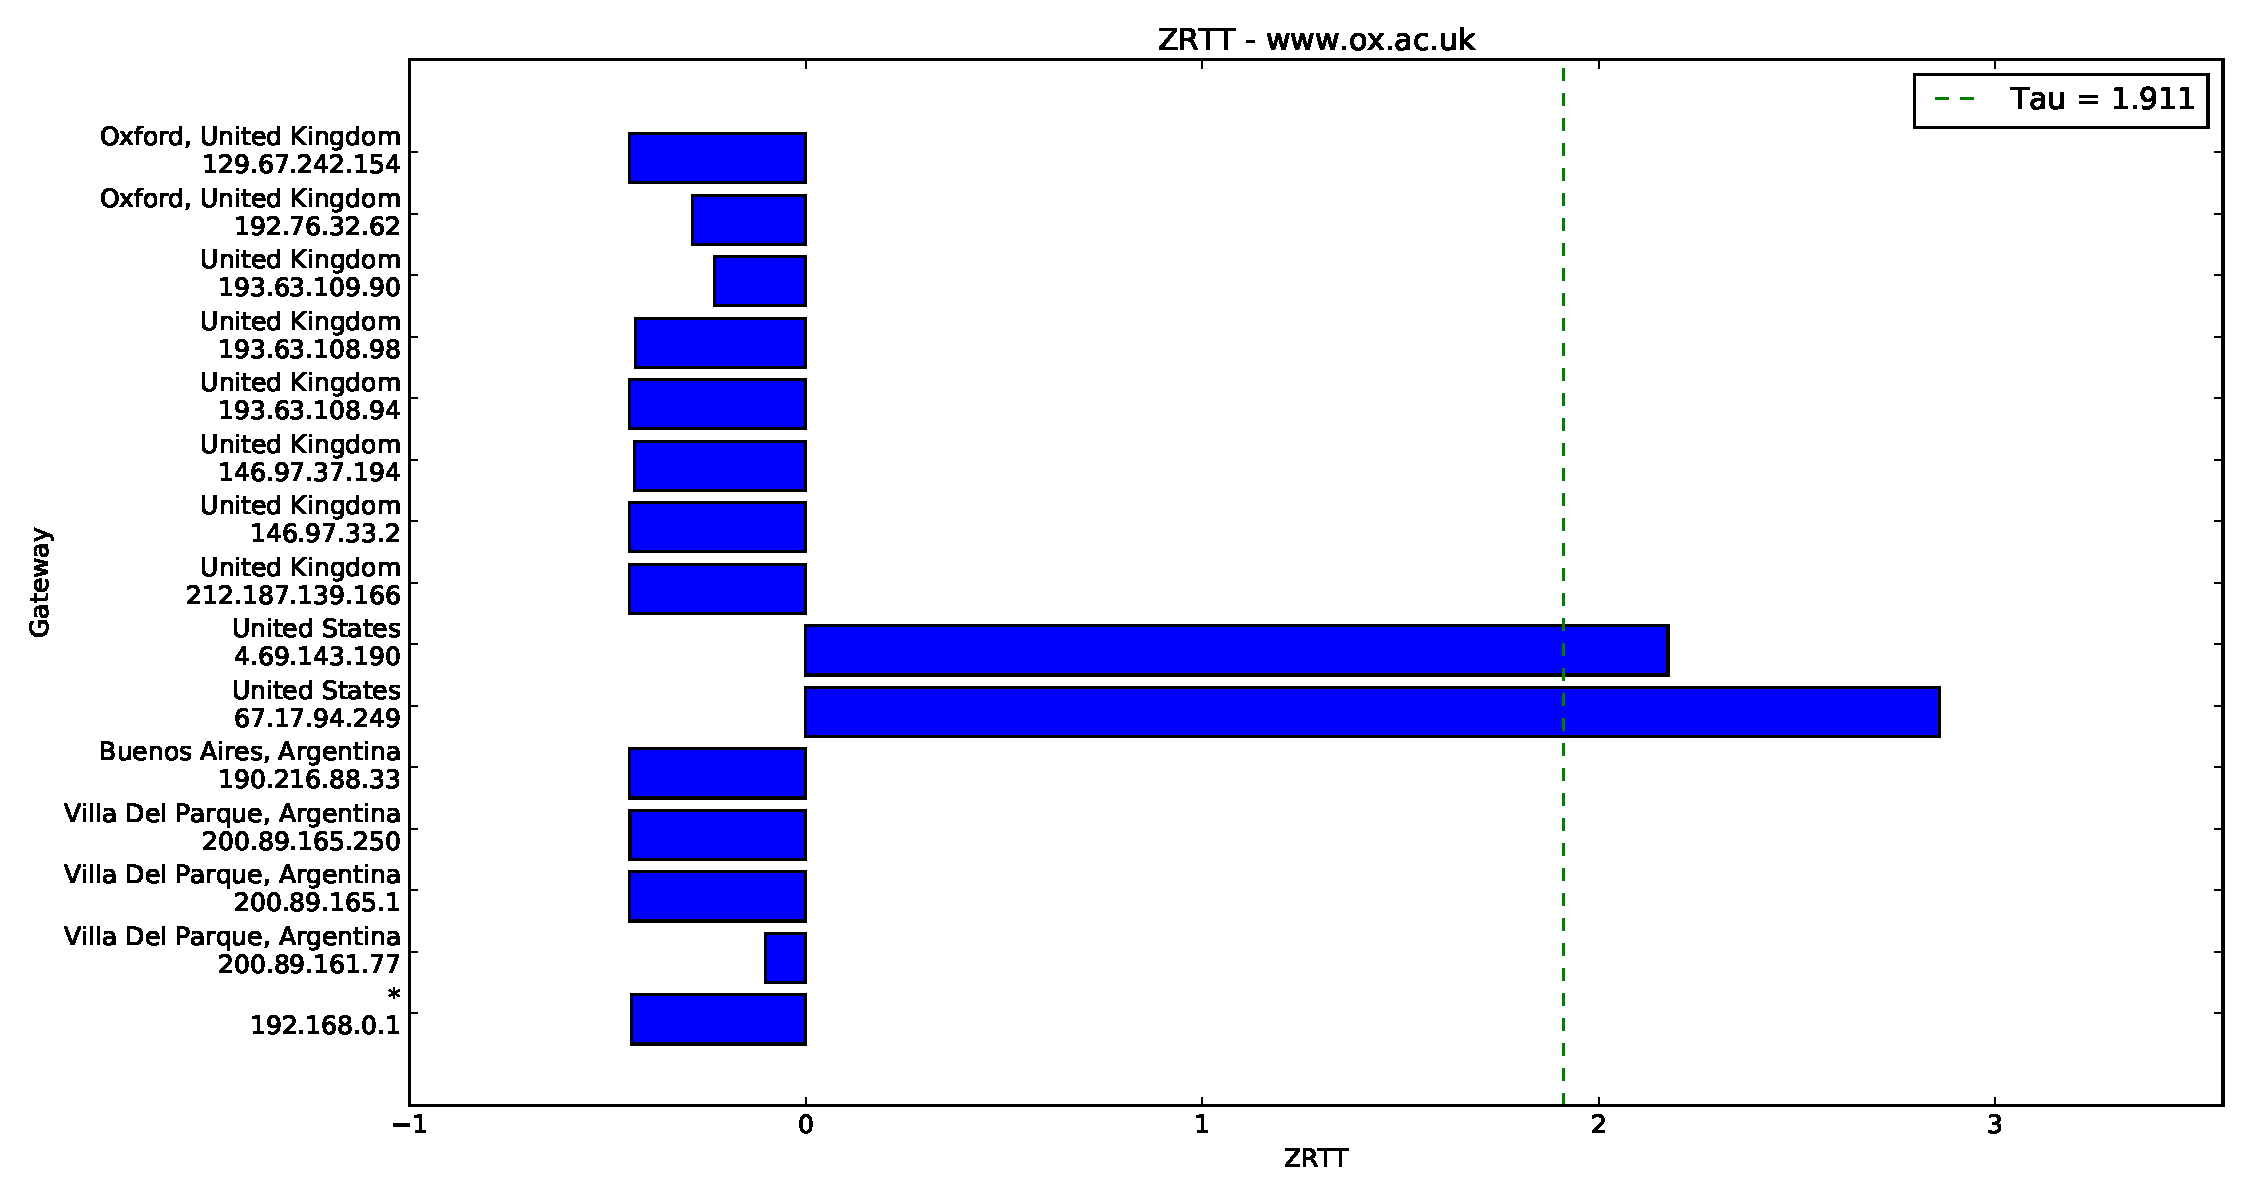
\includegraphics[width=8.5cm]{img/grafico2-www-ox-ac-uk.pdf}
    \caption{\normalfont ZRTTs entre saltos.}
\end{figure}

\begin{figure}[H]
    \centering
    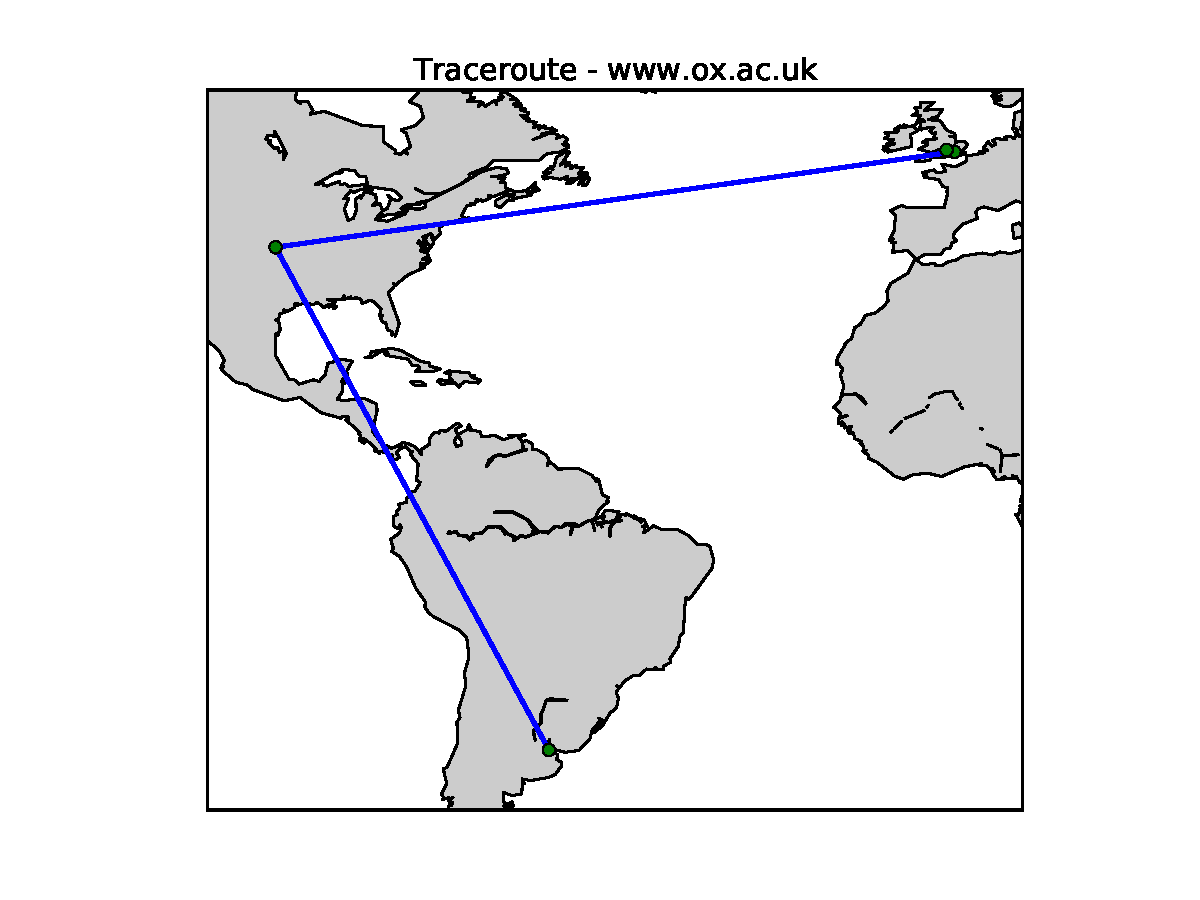
\includegraphics[width=8.5cm]{img/grafico3-www-ox-ac-uk.pdf}
    \caption{\normalfont Ubicación geográfica estimada de la ruta tomada.}
\end{figure}

Al realizar el traceroute, el porcentaje de saltos que no respondió los time exceeded fue de 38.09\% (exactamente 8 de 21). En términos de saltos que sí responden, la ruta tiene 13 nodos, incluyendo el router correspondiente a la red desde la cual se realizó el experimento.

Como se ve en los gráficos, se pueden observar dos \textit{outlier} entre los saltos efectuados, correspondientes a los enlaces entre Argentina - Estados Unidos y Estados Unidos - Inglaterra. Efectivamente, estos son los únicos dos enlaces intercontinentales que se encuentran entre el origen y el destino, y nuestro modelo pudo detectarlos. Al igual que en varios de nuestros experimentos, los paquetes pasan por Estados Unidos para llegar a destino.

Además, se puede observar en el gráfico de las ubicaciones geográficas que en el camino hasta llegar hasta la Universidad de Oxford, el paquete pasa por otra ciudad ubicada en Inglaterra. Luego de varios experimentos con otras universidades cercanas, podemos predecir que esta ciudad se trata de Londres, donde, efectivamente, se encuentra un enlace submarino con Estados Unidos.



\section{Conclusión}

\PARstart Observamos algunos de los comportamientos anómalos mencionados en Jobs 2012\cite{anomalias}: el más ubicuo es el primero descripto en el paper, donde ciertos nodos no responden los \textit{Time exceeded}. 
También observamos el caso donde routers \textit{MPLS} no aparecen en la \textit{traceroute}.

\par En el experimento a la Universidad de Laval se observa una gran cantidad de RTTs entre saltos negativos.
Esto puede ser un ejemplo de la anomalía "False Roundtrip Times" mencionada en el paper: la ruta de vuelta es asimétrica, por lo que los paquetes de \textit{Time exceeded} son forwardeados hacia delante en la ruta antes de volver al origen, resultando en RTTs relativos negativos.

\par Una anomalía que se observa frecuentemente al realizar \textit{traceroutes} pero que no se presentó en ninguno de los experimentos es la de \textit{missing destination}.
El hecho de que no se haya incurrido en ésta puede deberse a una mera coincidencia, o puede ser una consecuencia del tipo de destinos elegidos: por la consigna, todos son universidades.
La típica causa de la anomalía es un \textit{firewall} bloqueando los paquetes \textit{ICMP} al destino; es posible que este \textit{setup} sea preferido por los servers comerciales e ignorado por las instituciones académicas, quizás debido a un mayor enfoque en la \textit{performance} por parte de los primeros.

\par Frecuentemente la herramienta geográfica utilizada realizó estimaciones incorrectas en nodos cercanos a y coincidentes con cables submarinos.
Esta anomalía no es mencionada en el paper ya que no se enfocan en el aspecto geográfico de las \textit{traceroutes}.

\par Si las estimaciones se realizan a partir de ubicaciones iniciales conocidas, y de un análisis estadístico de las ubicaciones conocidas y estimados de los vecinos de los nodos desconocidos, es de esperar que los errores se concentren en las conexiones entre regiones distintas, como en el caso de los cables submarinos.

\par Ningún experimento presentó falsos negativos, y sólo uno resultó en un falso negativo.
Si bien era una de las rutas más largas, no consideramos que éste sea el factor fundamental en la predicción fallida; el experimento a la Universidad de \={O}saka (a una distancia similar) fue satisfactorio.
En el caso del experimento a la Universidad de Alejandría, la ruta submarina mal clasificada era la más corta de todas las analizadas; la longitud de la ruta es un factor mucho menos influyente que su topología: una ruta consistente de pequeños saltos resultará en un $\tau$ mucho menor que una de igual longitud pero con una conexión submarina cubriendo gran parte de su extensión.

\par En el único experimento donde el modelo falló, un cálculo distinto del $\tau$ hubiera sido irrelevante ya que el ZRTT de la conexión marítima mal clasificada es negativo; el falso negativo no podría subsanarse sin un extremo número de falsos positivos.


%----------------------------------------------------------------------

\begin{thebibliography}{1}

%\bibitem{enunciado}
%C\'atedra de Teor\'ia de las Comunicaciones\\
%\newblock {\em Primer trabajo pr\'actico}\\
%\newblock Primer cuatrimestre $2013$

%\bibitem{arp}
%RFC 826 - Ethernet Address Resolution Protocol\\
%\url{http://tools.ietf.org/html/rfc826}\\
%\newblock C. Plummer $1982$

%\bibitem{conflicto}
%RFC 5227 - IPv4 Address Conflict Detection\\
%\url{http://tools.ietf.org/html/rfc3927}\\
%\newblock S. Cheshire $2008$

%\bibitem{link}
%RFC 3927 - Configuration of IPv4 Link-Local Addresses\\
%\url{http://tools.ietf.org/html/rfc3927}\\
%\newblock Cheshire, et al. $2005$

%\bibitem{patente}
%Method and apparatus for detecting a router that improperly responds to ARP requests\\
%\newblock US 7729292 B2\\
%\url{http://www.google.com/patents/US7729292}\\
%\newblock Stuart D. Cheshire y Joshua V. Graessley

\bibitem{scapy}
\texttt{Scapy}\\
\url{http://www.secdev.org/projects/scapy}

%\bibitem{dhcp}
%RFC 1531 - Dynamic Host Configuration Protocol\\
%\url{https://tools.ietf.org/html/rfc1531}

%\bibitem{tcp}
%\url{http://www.tcpdump.org}

\end{thebibliography}


\end{document}

